\newcommand{\shortened}[1]{\color{black} #1\xspace\color{black}}
\newcommand{\newlyadded}[1]{\color{black} #1\xspace\color{black}}
\newcommand{\fixed}[1]{\color{black} #1\xspace\color{black}}


\chapter{Selective Prediction Via Training Dynamics}
\label{ch:sptd}

\begin{paperref}
\normalfont
The contents of this chapter consist of research and results taken from: \citet{rabanser2022selective}: \emph{\bibentry{rabanser2022selective}}
\end{paperref}

\section*{Summary}

Selective Prediction is the task of rejecting inputs a model would predict incorrectly on. This involves a trade-off between input space coverage (how many data points are accepted) and model utility (how good is the performance on accepted data points). Current methods for selective prediction typically impose constraints on either the model architecture or the optimization objective; this inhibits their usage in practice and introduces unknown interactions with pre-existing loss functions. In contrast to prior work, we show that state-of-the-art selective prediction performance can be attained solely from studying the (discretized) training dynamics of a model. We propose a general framework that, given a test input, monitors metrics capturing the instability of predictions from intermediate models (\ie checkpoints) obtained during training w.r.t. the final model's prediction. In particular, we reject data points exhibiting too much disagreement with the final prediction at late stages in training. The proposed rejection mechanism is domain-agnostic (\ie it works for both discrete and real-valued prediction) and can be flexibly combined with existing selective prediction approaches as it does not require any train-time modifications. Our experimental evaluation on image classification, regression, and time series problems shows that our method beats past state-of-the-art accuracy/utility trade-offs on typical selective prediction benchmarks.


\section{Introduction}

Machine learning (ML) is increasingly deployed in high-stakes decision-making environments with strong reliability and safety requirements. One of these requirements is the detection of inputs for which the ML model produces an erroneous prediction. This is particularly important when deploying deep neural networks (DNNs) for applications with low tolerances for \fps (\ie classifying with a wrong label), such as healthcare~\citep{challen2019artificial, mozannar2020consistent}, self-driving~\citep{ghodsi2021generating}, and law~\citep{vieira2021understanding}.
This problem setup is captured by the Selective Prediction (SP) framework, which introduces an accept/reject function (a so-called \emph{gating mechanism}) to abstain from predicting on individual test points in the presence of high prediction uncertainty~\citep{geifman2017selective}. 
Specifically, SP aims to (i) only accept inputs on which the ML model would achieve high utility, while (ii) maintaining high coverage (\ie correctly accepting as many inputs as possible).

Current selective prediction techniques 
take one of two directions: (i) augmentation of the architecture of the underlying ML model~\citep{geifman2019selectivenet}; or (ii) training the model using a purposefully adapted loss function~\citep{liu2019deep, huang2020self, gangrade2021selective}. 
The unifying principle behind these methods is to modify the training stage in order to accommodate selective prediction. While many ad-hoc experimentation setups are amenable to these changes, productionalized environments often impose data pipeline constraints which limit the applicability of existing methods. Such constraints include, but are not limited to, data access revocation, high (re)-training costs, or pre-existing architecture/loss modifications whose interplay with selective prediction adaptations are unexplored. As a result of theses limitations, selective prediction approaches are hard to deploy in production environments.

We instead show that \textit{ these modifications are unnecessary}. That is, our method, which \textbf{establishes new SOTA results for selective prediction} across a variety of datasets, not only outperforms existing work but \textbf{our method can be easily applied on top of all existing models}, unlike past methods. Moreover, our method is not restricted to classification problems but can be applied for real-valued prediction problems, too, like regression and time series prediction tasks. This is an important contribution as a majority of recent selective prediction approaches have solely focused on improving selective \emph{classification}.

\begin{figure*}[t]
    \centering
    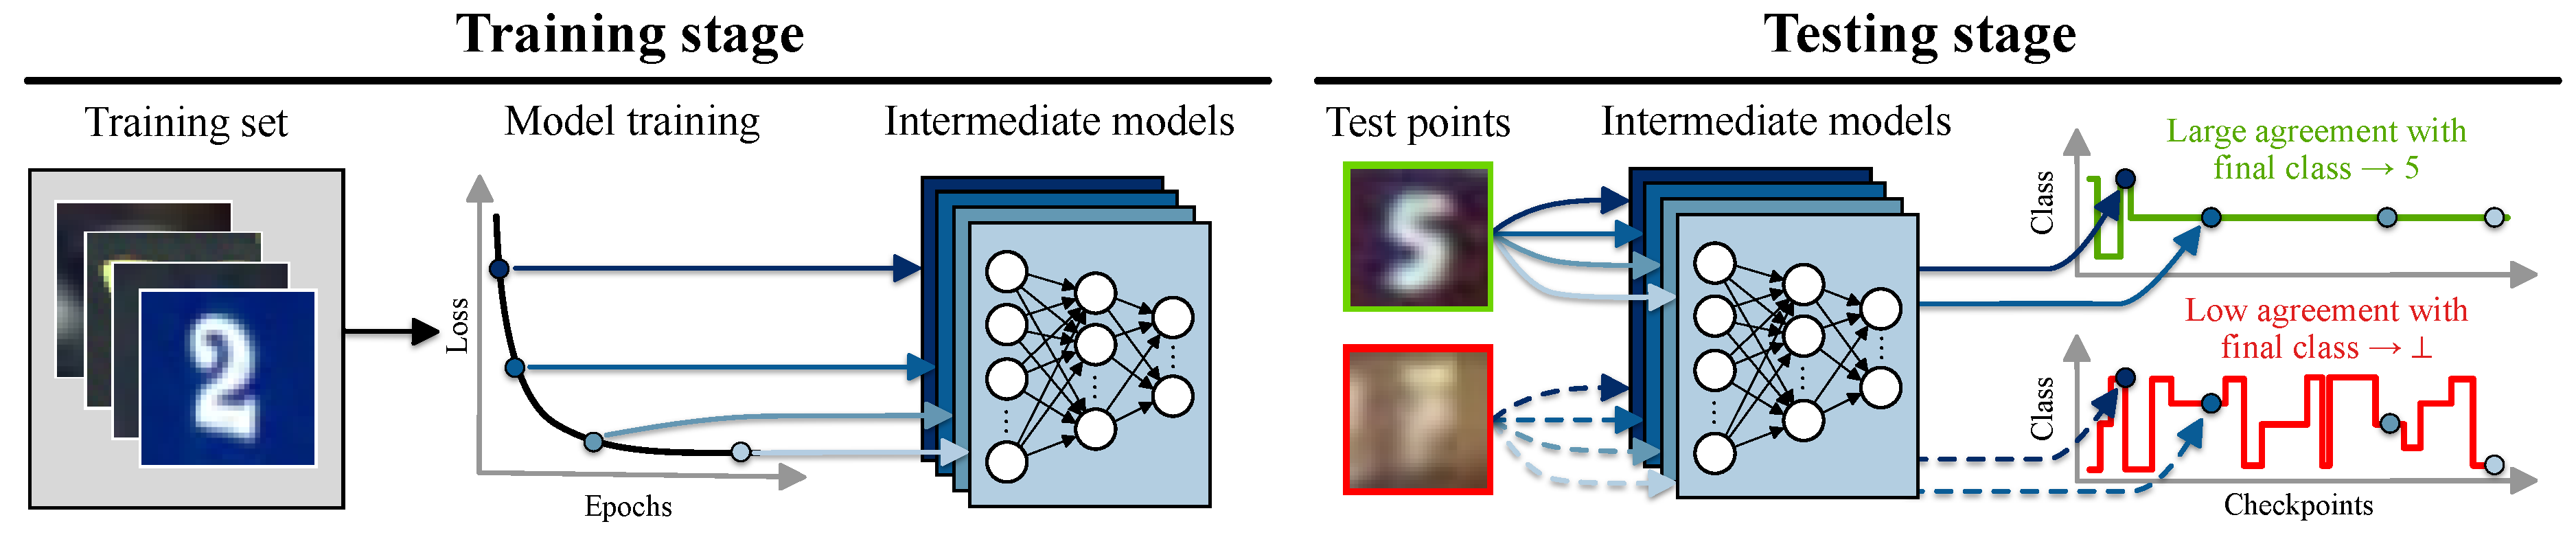
\includegraphics[width=0.97\linewidth]{figs/sptd/nntd.pdf}
    \caption[Our proposed \sptd method for a classification example]{\textbf{Our proposed \sptd method for a classification example}. We store checkpoints of intermediate models during model training. At inference time, given a test input, we compute various metrics capturing the stability of intermediate predictions with respect to the final model prediction. Data points with high stability are accepted, data points with low stability are rejected.}
    \label{fig:nntd_overview}
\end{figure*}

Our approach builds on the following observation: typical DNNs are trained using an iterative optimization procedure, \eg using Stochastic Gradient Descent (SGD). Due to the sequential nature of this optimization process, as training goes on, the optimization process yields a sequence of intermediate models. \newlyadded{Current selective prediction methods rely only on the final model, ignoring valuable statistics available from the model’s training sequence.}
In this work, however, we propose to take advantage of the information contained in these optimization trajectories for the purpose of selective prediction. By studying the usefulness of these trajectories, we observe that instability in SGD convergence is often indicative of high aleatoric uncertainty (\ie irreducible data noise such as overlap between distinct data classes). Furthermore, past work on example difficulty~\citep{jiang2020characterizing,toneva2018empirical,hooker2019compressed,agarwal2020estimating} has highlighted faster convergence as indicative of easy-to-learn training examples (and conversely slow convergence of hard-to-learn training examples). We hypothesize that such training time correlations with uncertainty also hold for test points and studying how test time predictions evolve over the intermediate checkpoints is useful for reliable uncertainty quantification.

With this hypothesis, we derive the first framework for \textbf{S}elective \textbf{P}rediction based on neural network \textbf{T}raining \textbf{D}ynamics~(\sptd, see Figure~\ref{fig:nntd_overview} for an example using a classification setup). Through a formalization of this particular neural network training dynamics problem, we first note that a useful property of the intermediate models' predictions for a test point is whether they converge ahead of the final prediction. This convergence can be measured by deriving a prediction instability score measuring how strongly predictions of intermediate models agree with the final model. While the exact specifics of how we measure instability differs between domains (classification vs regression), our resulting score generalizes across application domains and measures weighted prediction instability. This weighting allows us to emphasize instability late in training which we deem indicative of points that should be rejected. Note that this approach is transparent w.r.t. the training stage: our method only requires that intermediate checkpoints were recorded when a model was trained, which is an established practice (especially when operating in shared computing environments such as GPU clusters). Moreover, when compared to competing ensembling-based methods, such as Deep Ensembles~\citep{balaji2017uncertainty}, our approach can match the same inference-time cost while being significantly cheaper to train.

To summarize, our main contributions are as follows: 
\begin{enumerate}
    \item We present a motivating synthetic example using a linear model, showcasing the effectiveness of training dynamics information in the presence of a challenging classification task (Section~\ref{sec:method_intuition}). 
    \item We propose a novel method for selective prediction based on training dynamics (\sptd, Section~\ref{sec:method_overview}). To that end, we devise an effective scoring mechanism capturing weighted prediction instability of intermediate models with the final prediction for individual test points. Our methods allow for selective classification, selective regression, and selective time series prediction. Moreover, \sptd can be applied to all existing models whose checkpoints were recorded during training.
    \item We highlight an in-depth connection between our \sptd approach and forging (\cite{thudi2022necessity}, Section~\ref{sec:forging}), which has shown that optimizing a model on distinct datasets can lead to the same sequence of checkpoints. This connection demonstrates that our metrics can be motivated from a variety of different perspectives.
    \item We perform a comprehensive set of empirical experiments on established selective prediction benchmarks spanning over classification, regression, and time series prediction problems (Section~\ref{sec:emp_eval}). 
    Our results obtained from all instances of \sptd demonstrate highly favorable utility/coverage trade-offs, establishing new state-of-the-art results in the field at a fraction of the training time cost of competitive prior approaches. 
\end{enumerate}


\section{Background on Selective Prediction}
\label{sec:background_sptd}

\paragraph{Supervised Learning Setup.} Our work considers the standard supervised learning setup. We assume access to a dataset $D = \{(\bm{x}_i,y_i)\}_{i=1}^{M}$ consisting of $M$ data points $(\bm{x},y)$ with $\bm{x} \in \mathcal{X}$ and  $y \in \mathcal{Y}$. We refer to $\mathcal{X} := \mathbb{R}^d$ as the covariate space (or input/data space) of dimensionality $d$. For classification problems, we define $\mathcal{Y} := [C] = \{1, 2, \ldots, C\}$ as the label space consisting of $C$ classes. For regression and time series problems (such as demand forecasting) we instead define $\mathcal{Y} := \mathbb{R}$ and $\mathcal{Y} := \mathbb{R}^R$ respectively (with $R$ being the prediction horizon). All data points $(\bm{x},y)$ are sampled independently from the underlying distribution $p$ defined over the joint covariate and label spaces $\mathcal{X} \times \mathcal{Y}$. Our goal is to learn a prediction function $f : \mathcal{X} \rightarrow \mathcal{Y}$ which minimizes the risk $\mathcal{R}(f_{\bm{\theta}})$ with respect to the underlying data distribution $p$ and an appropriately chosen loss function $\ell : \mathcal{Y} \times \mathcal{Y} \rightarrow \mathbb{R}$. 
We can derive the optimal parameters $\hat{\bm{\theta}}$ via empirical risk minimization which approximates the true risk $\mathcal{R}(f_{\bm{\theta}})$ through sampling, thereby ensuring that $\bm{\theta}^* \approx \hat{\bm{\theta}}$ for a sufficiently large amount of samples:
\begin{align}
    \bm{\theta}^* & = \argmin_{\bm{\theta}} \mathcal{R}(f_{\bm{\theta}}) = \argmin_{\bm{\theta}} \mathbb{E}_{p(\bm{x},y)}[\ell(f_{\bm{\theta}}(\bm{x}),y)] \\ 
    \hat{\bm{\theta}} & = \argmin_{\bm{\theta}} \hat{\mathcal{R}}(f_{\bm{\theta}}) = \argmin_{\bm{\theta}} \frac{1}{M} \sum_{i=1}^{N} \ell(f_{\bm{\theta}}(\bm{x}_i),y_i)
\end{align}
In the following, we drop the explicit dependence of $f$ on $\bm{\theta}$ and simply denote the predictive function by $f$.

\paragraph{Selective Prediction Setup.} Selective prediction alters the standard supervised learning setup by introducing a rejection state~$\bot$ through a \textit{gating mechanism}~\citep{yaniv2010riskcoveragecurve}. In particular, such a mechanism introduces a selection function $g:\mathcal{X} \rightarrow \mathbb{R}$ which determines if a model should predict on a data point~$\bm{x}$. 
Given an acceptance threshold $\tau$, the resulting predictive model can be summarized as:
\begin{equation}
    (f,g)(\bm{x}) = \begin{cases}
  f(\bm{x})  & g(\bm{x}) \leq \tau \\
  \bot & \text{otherwise.}
\end{cases}
\end{equation}

\paragraph{Selective Prediction Evaluation Metrics.} Prior work evaluates the performance of a selective predictor $(f,g)$ based on two metrics: the \emph{coverage} of $(f,g)$ (\ie what fraction of points we predict on) and the \emph{selective utility} of $(f,g)$ on the accepted points. Note that the exact utility metric depends on the type of the underlying selective prediction task (e.g. accuracy for classification, $R^2$ for regression, and a quantile-based loss for time series forecasting). Successful SP methods aim to obtain both strong selective utility and high coverage. Note that these two metrics are at odds with each other: na\"ively improving utility leads to lower coverage and vice-versa. The complete performance profile of a model can be specified using the risk–coverage curve, which defines the risk as a function of coverage~\citep{yaniv2010riskcoveragecurve}. These metrics can be formally defined as: 
\begin{align}
    \text{coverage}(f,g) & = \frac{M_\tau}{M} \\
    \text{utility}(f,g) & = \sum_{ \{(\bm{x}, y) : g(\bm{x}) \leq \tau \} } u(f(\bm{x}), y)
\end{align}
Here, $u(\cdot, \cdot)$ corresponds to the specifically used utility function, $M_\tau = \sum_{i=1}^M \mathds{1}[\bm{x}_i : g(\bm{x}_i) \leq \tau]$ corresponds to the number of accepted data points at threshold $\tau$, and $\mathds{1}[\cdot]$ corresponds to the indicator function. We define the following utility functions to be used based on the problem domain:

\begin{enumerate}
    \item \textit{Classification}: We use accuracy on accepted points as our utility function for classification:
    \begin{equation}
        \text{Accuracy} = \frac{1}{M_\tau}\sum_{i=1}^{M_\tau} \mathds{1}[\bm{x}_i : f(\bm{x}_i) = y_i]
    \end{equation}
    \item \textit{Regression}: We use the coefficient of determination ($R^2$ score, which is a scaled version of the mean squared error) on accepted points as our utility function for regression:
     \begin{equation}
        R^2= 1 - \frac{\sum_{i=1}^{M_\tau} (f(\bm{x}_i) - y_i)^2}{\sum_{i=1}^{M_\tau} (y_i - \frac{1}{M_\tau}\sum_{j=1}^{M_\tau} y_j)^2}
    \end{equation}
    \item \textit{Time Series Forecasting}: We use the Mean Scaled Interval Score (MSIS)~\cite{gneiting2007strictly} on accepted series as our utility function for time series forecasting
    \begin{equation}
    \fontsize{7.75pt}{7.75pt}
    \text { MSIS }= \frac{1}{M_\tau R}\sum_{i=1}^{M_\tau} \frac{ \splitfrac{ \sum_{r=n+1}^{n+R}\left(u_{i,r}-l_{i,r}\right) +\frac{2}{\alpha}\left(l_{i,r}-y_{i,r}\right) \mathds{1}[y_{i,r}<l_{i,r}]}{ +\frac{2}{\alpha}\left(y_{i,r}-u_{i,r}\right)  \mathds{1}[y_{i,r}>u_{i,r}] } }{\frac{1}{n-m} \sum_{r=m+1}^n\left|y_{i,r}-y_{i,r-m}\right|}
    \end{equation}
    where $\alpha$ refers to a specific predictive quantile, $n$ to the conditioning length of the time series, $m$ to the length of the seasonal period, and $u_{i,r}$ and $l_{i,r}$ to the upper and lower bounds on the prediction range, respectively.
\end{enumerate}

\subsection{Past \& Related Work} 

\paragraph{Softmax Response Baseline (Classification).} The first work on selective classification was the softmax response (\sr) mechanism~\citep{hendrycks2016baseline, geifman2017selective}. A classification model typically has a softmax output layer which takes in unnormalized activations in $z_{i} \in \mathbb{R}^C$ (referred to as logits) from a linear model or a deep neural net. These activations are mapped through the softmax function which normalizes all entries 
\begin{equation}
    \sigma(\bm{z})_{i}=\frac{e^{z_{i}}}{\sum_{j=1}^{K} e^{z_{j}}}
\end{equation}
to the interval $[0,1]$ and further ensures that $\sum_{i=1}^{C} \sigma(\bm{z})_{i} = 1$. As a result, the softmax output can be interpreted as a conditional probability distribution which we denote $f(y|\bm{x})$.
The softmax response mechanism applies a threshold $\tau$ to the maximum response of the softmax layer: $\max_{y \in \mathcal{Y}}f(y|\bm{x})$. 
Given a confidence parameter $\delta$ and desired risk $\hat{\mathcal{R}}(f)$, \sr constructs $(f, g)$ with test error no larger than $\hat{\mathcal{R}}(f)$ with probability $\geq 1-\delta$. 
While this approach is simple to implement, it has been shown to produce over-confident results due to poor calibration of deep neural networks~\citep{guo2017calibration}.\footnote{Under miscalibration, a model's prediction frequency of events does not match the true frequency of events.} 

\paragraph{Loss Modifications (Mostly Classification).} 
The first work to deliberately address selective classification via architecture modification was SelectiveNet~\citep{geifman2019selectivenet}, which trains a model to jointly optimize for classification and rejection. A loss penalty is added to enforce a particular coverage constraint using a variant of the interior point method~\cite{potra2000interior} which is often used for solving linear and non-linear convex optimization problems. To optimize selective accuracy over the full coverage spectrum in a single training run, Deep Gamblers~\citep{liu2019deep} transform the original $C$-class problem into a $(C + 1)$-class problem where the additional class represents model abstention. \shortened{A similar approach is given by Self-Adaptive Training (\sat)~\citep{huang2020self} which also uses a $(C+1)$-class setup but instead incorporates an exponential average of intermediate predictions into the loss function.} Other similar approaches include: performing statistical inference for the marginal prediction-set coverage rates using model ensembles~\citep{feng2021selective}, confidence prediction using an earlier snapshot of the model~\citep{geifman2018bias}, estimating the gap between classification regions corresponding to each class~\citep{gangrade2021selective}, and complete precision by classifying only when models consistent with the training data predict the same output~\citep{khani2016unanimous}. 

\paragraph{Uncertainty Quantification (Classification + Regression).} 
It was further shown by~\citep{balaji2017uncertainty, zaoui2020regression} that deep model ensembles (\ie a collection of multiple models trained with different hyper-parameters until convergence) can provide state-of-the-art uncertainty quantification, a task closely related to selective prediction. This however raises the need to train multiple models from scratch. \shortened{To reduce the cost of training multiple models, \citep{gal2016dropout} proposed abstention based on the variance statistics from several dropout \cite{srivastava2014dropout} enabled forward passes at test time.} Another popular technique for uncertainty quantification, especially for regression and time series forecasting, is given by directly modeling the output distribution~\citep{alexandrov2019gluonts} in a parametric fashion. Training with a parametric output distribution however can lead to additional training instability, often requiring extensive hyper-parameter tuning and distributional assumptions. On the other hand, our approach does not require any architecture or other training-time modifications. \newlyadded{Finally, we note that selective prediction and uncertainty are also strongly related to the field of automated model evaluation which relies on the construction a proximal prediction pipeline of the testing performance without the presence of ground-truth labels~\citep{peng2023came,peng2024energy}.}


\paragraph{Training Dynamics Approaches (Classification).} Checkpoint and snapshot ensembles \citep{huang2017snapshot, chen2017checkpoint} constitute the first usage of training dynamics to boost model utility. Our work is closest in spirit to recent work on dataset cartography~\citep{swayamdipta2020dataset} which relies on using training dynamics from an example difficulty viewpoint by considering the variance of logits. However, their approach does not consider selective prediction and further requires access to true label information (which is not available in the selective prediction setting). Recent work on out-of-distribution detection~\citep{adila2022understanding}, a closely related yet distinct application scenario from selective prediction, harness similar training dynamics based signals.


\paragraph{Example Difficulty.}
\label{sec:example_diff}

A related line of work to selective prediction is identifying \emph{difficult} examples, or how well a model can generalize to a given unseen example. Recent work~\cite{jiang2020characterizing} has demonstrated that the probability of predicting the ground truth label with models trained on data sub-samples of different sizes can be estimated via a per-instance empirical consistency score. Unlike our approach, however, this requires training a large number of models. 
Example difficulty can also be quantified through the lens of a forgetting event ~\cite{toneva2018empirical} in which the example is misclassified after being correctly classified. Instead, the metrics that we introduce in Section~\ref{sec:method}, are based on the disagreement of the label at each checkpoint with the final predicted label. Other approaches estimate the example difficulty by: 
prediction depth of the first layer at which a $k$-NN classifier correctly classifies an example~\citep{baldock2021deep}, the impact of quantization and compression on model predictions of a given sample~\citep{hooker2019compressed}, and estimating the leave-one-out influence of each training example on the accuracy of an algorithm by using influence functions~\citep{feldman2020neural}. 
Closest to our method, the work of \cite{agarwal2020estimating} utilizes gradients of intermediate models during training to rank examples by  difficulty. In particular, they average pixel-wise variance of gradients for each given input image. 
Notably, this approach is more costly and less practical than our approach and also does not study the utility/coverage trade-off which is of paramount importance to selective prediction.

\newlyadded{
\paragraph{Disagreement.} Our \sptd method heavily relies on the presence of disagreements between intermediate models. Past work on (dis-)agreement has studied the connection between generalization and disagreement of full SGD runs \citep{jiang2021assessing} as well as correlations between in-distribution and out-of-distribution agreement across models \citep{baek2022agreement}.
}

\section{Selective Prediction via Neural Network Training Dynamics}
\label{sec:method}

We now introduce our selective prediction algorithms based on neural network training dynamics. We start by presenting a motivating example showcasing the effectiveness of analyzing training trajectories for a linear classification problem. Following this, we formalize our selective prediction scoring rule based on training-time prediction disagreements. We refer to the class of methods we propose as \sptd.

\subsection{Method Intuition: Prediction Disagreements Generalize Softmax Response}
\label{sec:method_intuition}

\begin{figure*}
    \centering
    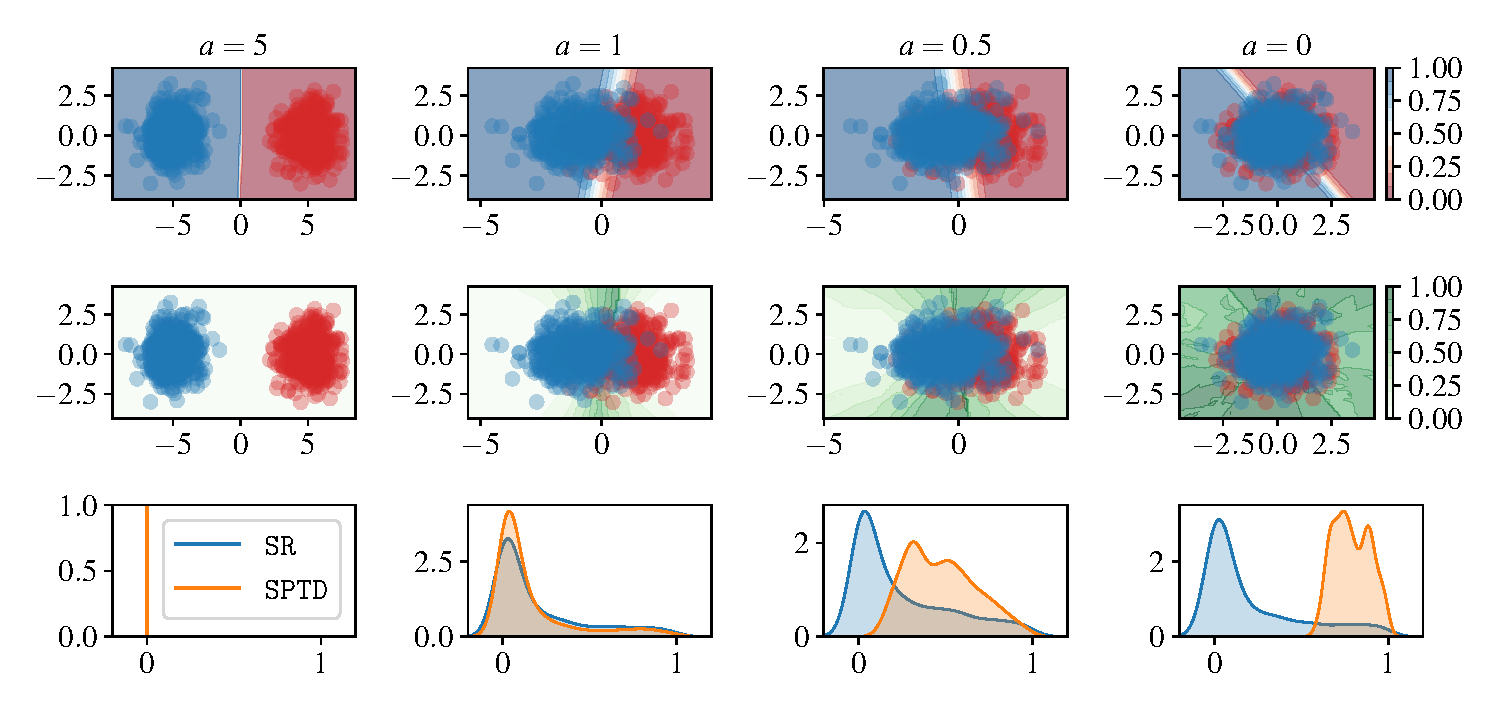
\includegraphics[width=0.97\linewidth]{figs/sptd/gaussians_anom2.pdf}
    \caption[Synthetic example of anomaly scoring based on \sr vs \sptd.]{\textbf{Synthetic example of anomaly scoring based on \sr vs \sptd}. The first row shows a test set from the generative Gaussian model as well as the learned decision boundary separating the two Gaussians. For small $a$, the decision boundary is overconfident. The second row shows the same data set but instead depicts the scores yielded by applying \sptd to the full domain. \sptd highlights rightful rejection regions more clearly than the overconfident \sr score: larger regions are flagged as exhibiting noisy training dynamics (with stronger shades of green indicating stronger disagreement) as $a \rightarrow 0$. The bottom row shows the distribution of the \sr and \sptd scores, clearly showing that \sptd leads to improved uncertainty under stronger label ambiguity.}
    \label{fig:gauss}
\end{figure*}


Stochastic iterative optimization procedures, such as Stochastic Gradient Descent (SGD), yield a sequence of models that is iteratively derived by minimizing a loss function $\ell(\cdot,\cdot)$ on a randomly selected mini-batch $(\bm{X}_i, \bm{y}_i)$ from the training set. The iterative update rule can be expressed as
\begin{equation}
    \bm{\theta}_{t+1} = \bm{\theta}_{t} - \nu \frac{\partial \ell(f(\bm{X}_i), \bm{y}_i)}{\partial \bm{\theta}_{t}},
\end{equation}
where the learning rate $\nu$ controls the speed of optimization and $t \in \{1,\ldots,T\}$ represents a particular time-step during the optimization process.

\looseness=-1
Current methods for selective prediction disregard the properties of this iterative process and only rely on the final set of parameters $\bm{\theta}_{T}$. However, the optimization trajectories contain information that we can use to determine prediction reliability. In particular, on hard optimization tasks, the presence of stochasticity from SGD and the potential ambiguity of the data often leads to noisy optimization behavior. As a result, intermediate predictions produced over the course of training might widely disagree in what the right prediction would be for a given data point. Our class of selective prediction approaches explicitly make use of these training dynamics by formalizing rejection scores based on the observed frequency of prediction disagreements with the final model throughout training.

To illustrate and reinforce this intuition that training dynamics contain meaningfully more useful information for selective prediction than the final model, we present a synthetic logistic regression example. First, we generate a mixture of two Gaussians each consisting of $1000$ samples: $D = \{(\bm{x}_i,0)\}_{i=1}^{1000} \cup \{(\bm{x}_j,1)\}_{j=1}^{1000}$ where $\bm{x}_i \sim \mathcal{N}(\begin{bmatrix}a & 0\end{bmatrix}^\top,\ \bm{I})$ and $\bm{x}_j \sim \mathcal{N}(\begin{bmatrix}-a & 0\end{bmatrix}^\top,\ \bm{I})$. Note that $a$ controls the distance between the two $2$-dimensional Gaussian clusters, allowing us to specify the difficulty of the learning task. Then, we train a linear classification model using SGD for $1000$ epochs for each $a \in \{0,0.5,1,5\}$. Finally, we compute both the softmax response score (\sr) score, the typical baseline for selective classification, as well as our \sptd score (details in Section~\ref{sec:method_overview}).

We showcase the results from this experiment in Figure~\ref{fig:gauss}. We  see that if the data is linearly separable ($a=5$) the learned decision boundary is optimal and the classifier's built-in confidence score \sr reflects well-calibrated uncertainty. Moreover, the optimization process is stable as \sptd yields low scores over the full domain. However, as we move the two Gaussians closer together (\ie by reducing $a$) we see that the \sr baseline increasingly suffers from overconfidence: large parts of the domain are very confidently classified as either $0$ (red) or $1$ (blue) with only a small ambiguous region (white). However, the optimization trajectory is highly unstable with the decision boundary changing abruptly between successive optimization steps. \sptd identifies the region of datapoints exhibiting large prediction disagreement due to this training instability and correctly rejects them (as those are regions also subject to label ambiguity in this case). In summary, we observe that \sptd provides improved uncertainty quantification in ambiguous classification regions (which induce training instability) and reduces to the \sr solution as the classification task becomes easier. Hence, we expect \sptd to generalize \sr performance, which is supported by this logistic regression experiment.

\subsection{Method Overview: Measuring Prediction Instability During Training}
\label{sec:method_overview}

\begin{figure*}
\begingroup
    \begin{minipage}{0.48\textwidth}

    \begin{algorithm}[H]
    	\caption{\sptd for classification}\label{alg:sptd_class}
    	\begin{algorithmic}[1]
    	\Require Intermediate models $[f_1,\ldots,f_T]$, query point $\bm{x}$, weighting parameter $k \in [0,\infty)$.
        \For{$t \in [T]$}
            \State \algemph{\algorithmicif\ $f_t(\bm{x}) = f_T(\bm{x})$ \algorithmicthen\ $a_t \gets 0$ \algorithmicelse\ $a_t \gets 1$}
            \State $\ v_t \gets (\frac{t}{T})^k$
        \EndFor
    \State $g \gets \sum_{t} v_t a_t$
    \State \algorithmicif\ $g \leq \tau$ \algorithmicthen\ \fixed{$f(\bm{x}) = f_T(\bm{x})$} \algorithmicelse\ $f(\bm{x}) = \bot$
    	\end{algorithmic}
    \end{algorithm}
    
    \end{minipage}
    \hfill
    \begin{minipage}{0.48\textwidth}

    \begin{algorithm}[H]
    	\caption{\sptd for regression}\label{alg:sptd_regr}
    	\begin{algorithmic}[1]
    	\Require Intermediate models $[f_1,\ldots,f_T]$, query point $\bm{x}$, weighting parameter $k \in [0,\infty)$. 
        \For{$t \in [T]$}
            \State \algemph{$a_t \gets ||f_t (\bm{x}) - f_T (\bm{x})||$}
            \State $\ v_t \gets (\frac{t}{T})^k$
        \EndFor
    \State $g \gets \sum_{t} v_t a_t$
    \State \algorithmicif\ $g \leq \tau$ \algorithmicthen\ \fixed{$f(\bm{x}) = f_T(\bm{x})$} \algorithmicelse\ $f(\bm{x}) = \bot$
    	\end{algorithmic}
    \end{algorithm}
    
    \end{minipage}

    \vspace{-10pt}
\endgroup
\end{figure*}

We proceed to describe the statistics we collect from intermediate checkpoints which we later devise our scores for deciding which inputs to reject on. The objective of these statistics is to capture how unstable the prediction for a datapoint was over the training checkpoints. Let $[f_1,f_2,\ldots, f_T]$ be a sequence of intermediate checkpoints, and $\mathcal{D} = D_\text{train} \cup D_\text{test}$ be the set of all data points. We define a prediction disagreement score at time $t \in \{1,\ldots,T\}$ as some function $a_t: \mathcal{X} \rightarrow \mathbb{R}^+$ with $a_t(\bm{x}) = 0$ if $f_t(\bm{x}) = f_T(\bm{x})$. Note that the exact $a_t(\cdot)$ we use depends on the problem domain (classification vs regression) and we define our choices below. In the following, when conditioning on $\bm{x}$ is understood from context, we drop the explicit dependence on $\bm{x}$ and write $a_t$.

For a fixed data point $\bm{x}$, our approach takes a given sequence of prediction disagreements $[a_1,\ldots,a_T]$ and associates a weight $v_t$ to each disagreement $a_t$ to capture how severe a disagreement at step $t$ is. To derive this weighting we ask: How indicative of $\bm{x}$ being incorrectly classified is a disagreement at step $t$? Related work in the example difficulty literature (see Section~\ref{sec:example_diff} for details) found that easy-to-optimize samples are learned early in training and converge faster. While prior work specifically derived these convergence insights for training points only, the novelty of our method is to show such conclusions for training points also generalize to test points. Hence, we propose to use the weighting $v_t = (\frac{t}{T})^k$ for $k \in [0,\infty)$ to penalize late prediction disagreements as more indicative of a test point we will not predict correctly on. With this weighting, our methods compute a weighted sum of the prediction disagreements, which effectively forms our selection function $g(\cdot)$: 
\begin{equation}
    \label{eq:score}
    g(\bm{x}) = \sum_{t} v_t a_t(\bm{x})    
\end{equation}

\paragraph{Instability for Classification.} For discrete prediction problems (\ie classification) we define the label disagreement score as $a_t = 1- \delta_{f_t(\bm{x}),f_T(\bm{x})}$ where $\delta$ is the Dirac-delta function: $a_t$ is hence $1$ if the intermediate prediction $f_t$ at checkpoint $t$ disagrees with the final prediction $f_T$ for $\bm{x}$, else $0$. The resulting algorithm using this definition of $a_t$ for classification is given in Algorithm~\ref{alg:sptd_class}. We remark that continuous metrics such as the maximum softmax score, the predictive entropy (\ie the entropy of the predictive distribution $f(y|\bm{x})$), or the gap between the two most confident classes could be used as alternate measures for monitoring stability (see Appendix~\ref{sec:alt_scores} for a discussion). However, these measures only provide a noisy proxy and observing a discrete deviation in the predicted class provides the most direct signal for potential mis-classification.

\paragraph{Instability for Regression.} One key advantage of our method over many previous ones is that it is applicable to \emph{any} predictive model, including regression. Here, we propose the following prediction disagreement score measuring the distance of intermediate predictions to the final model's prediction: $a_t = ||f_t (\bm{x}) - f_T (\bm{x})||$.\footnote{We explored a more robust normalization by averaging predictions computed over the last $l$ checkpoints: $a_t = ||f_t (\bm{x}) - \frac{1}{n}\sum_{c \in \{T-l, T-l+1, \ldots, T \}} f_c (\bm{x})||$. Across many $l$, we found the obtained results to be statistically indistinguishable from the results obtained by normalizing w.r.t. the last checkpoint $f_T$.} The resulting algorithm using this definition of $a_t$ for regression is given in Algorithm~\ref{alg:sptd_regr}. We again highlight the fact that Algorithm~\ref{alg:sptd_regr} only differs from Algorithm~\ref{alg:sptd_class} in the computation of the prediction disagreement $a_t$ (line 2 highlighted in both algorithms).

\begin{algorithm}[t]
    \caption{\sptd for time series forecasting}\label{alg:sptd_ts}
    \begin{algorithmic}[1]
    \Require Intermediate models $[f_1,\ldots,f_T]$, query point $\bm{x}$, weighting $k \in [0,\infty)$, prediction horizon $R$. 
    \For{$t \in [T]$}
        \For{$r \in [R]$}
            \State $a_{t,r} \gets ||f_{t}(\bm{x})_r - f_{T}(\bm{x})_r||$
        \EndFor
        \State $v_t \gets (\frac{t}{T})^k$
    \EndFor
\State $g \gets \sum_r\sum_{t} v_t a_{t,r}$
\State \algorithmicif\ $g \leq \tau$ \algorithmicthen\ $f(\bm{x}) = L$ \algorithmicelse\ $f(\bm{x}) = \bot$
    \end{algorithmic}
\end{algorithm}

\paragraph{Instability for Time Series Prediction.} We can further generalize the instability sequence used for regression to time series prediction problems by computing the regression score for all time points on the prediction horizon. In particular, we compute $a_{t,r} = ||f_{t}(\bm{x})_r - f_{T}(\bm{x})_r||$ for all $r \in \{1,\ldots,R\}$. Recall that for time series problems $f_{t}(\bm{x})$ returns a vector of predictions $y \in \mathbb{R}^R$ and we use the subscript $r$ on $f_{t}(\bm{x})_r$ to denote the vector indexing operation. Our selection function is then given by computing Equation~\ref{eq:score} for each $r$ and summing up the instabilities over the prediction horizon: $g(\bm{x}) = \sum_r\sum_{t} v_t a_{t,r}(\bm{x})$. The full algorithm therefore shares many conceptual similarities with Algorithm~\ref{alg:sptd_regr} and we provide the detailed algorithm as part of Algorithm~\ref{alg:sptd_ts}. Note that the presented generalization for time series is applicable to any setting in which the variability of predictions can be computed. As such, this formalism can extend to application scenarios beyond time series prediction such as object detection or segmentation.

\subsection{Selective Prediction and Forging}
\label{sec:forging}

\begin{contriback}
This subsection was written with Anvith Thudi. Both Stephan and Anvith jointly developed the max score and the sum score. Anvith provided details on the connection to forging as well as the formalism of Lemma~\ref{lem:prob_accept}.
\end{contriback}

While our \sptd method is primarily motivated from the example difficulty view point, we remark that the scores \sptd computes to decide which points to reject can be derived from multiple different perspectives. To showcase this, we provide a formal treatment on the connection between selective classification and forging~\citep{thudi2022necessity}, which ultimately leads to the same selection function $g(\cdot)$ as above.

Previous work has shown that running SGD on different datasets could lead to the same final model~\citep{hardt2016train,bassily2020stability,thudi2022necessity}. For example, this is intuitive when two datasets were sampled from the same distribution. We would then expect that training on either dataset should not significantly affect the model returned by SGD. For our selective prediction problem, this suggests an approach to decide which points the model is likely to predict correctly on: identify the datasets that it could have been trained on (in lieu of the training set it was actually trained on). Any point from the datasets the model could have trained on would then be likely to be predicted on correctly by the model. Recent work on forging \cite{thudi2022necessity} solves this problem of identifying datasets the model could have trained on by brute-force searching through different mini-batches to determine if a mini-batch in the alternative dataset can be used to reproduce one of the original training steps. Even then, this is only a sufficient condition to show a datapoint could have plausibly been used to train: if the brute-force fails, it does not mean the datapoint could not have been used to obtain the final model. As an alternative, we propose to instead characterize the optimization behaviour of training on a dataset as a probabilistic necessary condition, i.e, a condition most datapoints that were (plausibly) trained on would satisfy based on training dynamics. Our modified hypothesis is then that the set of datapoints we optimized for (which contains the forgeable points) coincides significantly with the set of points the model predicts correctly on.


\subsubsection{A Framework for Being Optimized}
\label{ssec:reject_cond}

In this section we derive an upper-bound on the probability that a datapoint could have been used to obtain the model's checkpointing sequence. This yields a probabilistically necessary (though not sufficient) characterization of the points we explicitly optimized for. This bound, and the variables it depends on, informs what we characterize as "optimizing" for a datapoint, and, hence, our selective classification methods.

Let us denote the set of all datapoints as $\mathcal{D}$, and let $D \subset \mathcal{D}$ be the training set. We are interested in the setting where a model $f$ is plausibly sequentially trained on $D$ (e.g., with stochastic gradient descent). We thus also have access to a sequence of $T$ intermediate states for $f$, which we denote $[f_1,\ldots, f_T]$. In this sequence, note that $f_T$ is exactly the final model $f$. 

Now, let $p_{t}$ represent the random variable for outputs on $D$ given by an intermediate model $f_t$ where the outputs have been binarized: we have $0$ if the output agrees with the final prediction and $1$ if not. In other words, $p_{t}$ is the distribution of labels given by first drawing $\bm{x} \sim D$ and then outputting $1- \delta_{f_t(\bm{x}),f_T(\bm{x})}$ where $\delta$ denotes the Dirac delta function. Note that we always have both a well-defined mean and variance for $p_{t}$ as it is bounded. Furthermore, we always have the variances and expectations of $\{p_{t}\}$ converge to $0$ with increasing $t$: as $p_{T} = 0$ always and the sequence is finite convergence trivially occurs. To state this formally, let $v_t = \mathbb{V}_{\bm{x} \sim D}[p_{t}]$ and let $e_t = \mathbb{E}_{\bm{x} \sim D}[p_{t}]$ denote the variances and expectations over points in $D$. In particular, we remark that $e_T=0,\ v_T = 0$, so both $e_t$ and $v_t$ converge. More formally, for all $ \epsilon > 0$ there exists an $N \in \{1,\ldots, T\}$ such that $v_t < \epsilon$ for all $t > N$. Similarly, for all $\epsilon > 0$ there exists a (possibly different) $N \in \{1,\ldots, T\}$ such that $e_t < \epsilon$ for all $t > N$.

However, the core problem is that we do not know how this convergence in the variance and expectation occurs. More specifically, if we knew the exact values of $e_t$ and $v_t$, we could use the following bound on the fraction of training data points producing a given $[a_1,\cdots,a_t]$ as a reject option for points that are not optimized for.  We consequently introduce the notation $[a_1,\ldots,a_T]$ where $a_t = 1- \delta_{f_t(\bm{x}),f_T(\bm{x})}$ which we call the "label disagreement (at $t$)". Note that the $a_t$ are defined with respect to a given input, while $p_t$ represent the distribution of $a_t$ over all inputs in $D$.

\begin{lemma}
\label{lem:prob_accept}
Given a datapoint $\bm{x}$,  let $\{a_1,\ldots,a_T\}$ where $a_t = 1- \delta_{f_t(\bm{x}),f_T(\bm{x})}$. Assuming not all $a_t = e_t$ then the probability $\bm{x} \in D$ is  $\leq \min_{v_t~s.t~a_t \neq e_t}  \frac{v_t}{|a_t - e_t|^2}$.
\end{lemma}
\begin{proof}
By Chebyshev's inequality we have the probability of a particular sequence $\{a_1,\ldots,a_T\}$ occurring for a training point is $\leq \frac{v_t}{|a_t - e_t|^2}$ for every $t$ (a bound on any of the individual $a_t$ occurring as that event is in the event $|p_t - e_t| \geq |a_t - e_t|$ occurs). By taking the minimum over all these upper-bounds we obtain our upper-bound.
\end{proof}

We do not guarantee Lemma~\ref{lem:prob_accept} is tight. Though we do take a minimum to make it tighter, this is a minimum over inequalities all derived from Chebyshev's inequality\footnote{One could potentially use information about the distribution of points not in $D$ to refine this bound.}. Despite this potential looseness, using the bound from Lemma~\ref{lem:prob_accept}, we can design a na\"ive selective classification protocol based on the "optimized = correct (often)" hypothesis and use the above bound on being a plausible training datapoint as our characterization of optimization; for a test input $\bm{x}$, if the upper-bound on the probability of being a datapoint in $D$ is lower than some threshold $\tau$ reject, else accept. However, the following question prevents us from readily using this method: \emph{How do $\mathbb{E}[p_{t}]$ and $\mathbb{V}[p_{t}]$ evolve during training?}

\looseness=-1
To answer this question, we propose to examine how the predictions on plausible training points evolve during training. Informally, the evolution of $\mathbb{E}[p_{t}]$ represents knowing how often we predict the final label at step $t$, while the evolution of $\mathbb{V}[p_{t}]$ represents knowing how we become more consistent as we continue training. Do note that the performance of this optimization-based approach to selective classification will depend on how unoptimized incorrect test points are. In particular, our hypothesis is that incorrect points often appear sufficiently un-optimized, yielding distinguishable patterns for $\mathbb{E}[p_{t}]$ and $\mathbb{V}[p_{t}]$ when compared to optimized points. We verify this behavior in Section~\ref{sec:emp_eval} where we discuss the distinctive label evolution patterns of explicitly optimized, correct, and incorrect datapoints.

\subsubsection{Last Disagreement Model Score For Discrete Prediction (\smax)}
\label{ssec:min_score}

Here, we propose a selective classification approach based on characterizing optimizing for a datapoint based off of Lemma~\ref{lem:prob_accept}. Recall the bound given in Lemma~\ref{lem:prob_accept} depends on expected values and variances for the $p_t$ (denoted $e_t$ and $v_t$ respectively). In Section~\ref{sec:emp_eval} we observe that $e_t$ quickly converge to $0$, and so by assuming $e_t = 0$ always\footnote{We tried removing this assumption and observed similar performance.} the frequentist bound on how likely a datapoint is a training point becomes $\min_{t~s.t~a_t = 1} \frac{v_t}{|a_t - e_t|^2}= \min_{t~s.t~a_t = 1}v_t$. Using this result for selective classification, we would impose acceptance if $\min_{t~s.t~a_t = 1}v_t \geq \tau$. Moreover, in Section~\ref{sec:emp_eval}, we further observe that $v_t$ monotonically decreases in a convex manner (after an initial burn-in phase). Hence, imposing $\min_{t~s.t~a_t = 1}v_t \geq \tau$ simply imposes a last checkpoint that can have a disagreement with the final prediction.

Based on these insights, we propose the following selective classification score: $s_{\max} = \max_{t~s.t~a_t = 1} \frac{1}{v_t}$. Note that this score directly follows from the previous discussion but flips the thresholding direction from $\min_{t~s.t~a_t = 1}v_t \geq \tau$ to $\max_{t~s.t~a_t = 1} \frac{1}{v_t} \leq \tau$ for consistency with the anomaly scoring literature~\citep{ruff2018deep}. Finally, we choose to approximate the empirical trend of $v_t$ as observed in Section~\ref{sec:emp_eval} with $v_t = 1 - t^k$ for $k \in [1,\infty)$. Based on the choice of $k$, this approximation allows us to (i) avoid explicit estimation of $v_t$ from validation data; and (ii) enables us to flexibly specify how strongly we penalize model disagreements late in training.

Hence, our first algorithm for selective classification is:
\begin{enumerate}
    \item Denote $L = f_T(\bm{x})$, i.e. the label our final model predicts.
    \item If $\exists t~s.t~a_t =1$ then compute $s_\text{max} = \max_{t~s.t~a_t = 1} \frac{1}{v_t}$ as per the notation in Section~\ref{ssec:reject_cond} (i.e $a_t = 1$ iff $f_t(x) \neq L$), else accept $\bm{x}$ with prediction $L$.
    \item If $s_\text{max} \leq \tau$ accept $\bm{x}$ with prediction $L$, else reject ($\bot$).
\end{enumerate}
Note once again, as all our candidate $\frac{1}{v_t}$ increase, the algorithm imposes a last intermediate model which can output a prediction that disagrees with the final prediction: hereafter, the algorithm must output models that consistently agree with the final prediction.

\subsubsection{Overall Disagreement Model Score (\ssum)}
\label{ssec:avg_score}

Note that the previous characterization of optimization, defined by the score \smax, could be sensitive to stochasticity in training and hence perform sub-optimally. That is, the exact time of the last disagreement, which \smax relies on, is subject to high noise across randomized training runs. In light of this potential limitation we propose the following "summation" algorithm which computes a weighted sum over training-time disagreements to get a more consistent statistic. Do note that typically to get a lower-variance statistic one would take an average, but multiplying by scalars can be replaced by correspondingly scaling the threshold we use. Hence, our proposed algorithm is:

\begin{enumerate}
     \item Denote $L = f_T(\bm{x})$, i.e. the label our final model predicts.
     \item If $\exists t~s.t~a_t =1$, compute $s_\text{sum} = \sum_{t=1}^T \frac{a_t}{v_t} $, else accept $\bm{x}$ with prediction $L$. 
     \item If $s_\text{sum} \leq \tau$ accept $\bm{x}$ with prediction $L$, else reject ($\bot$).
\end{enumerate}

Recalling our previous candidates for $v_t$, we have the \ssum places higher weight on late disagreements. This gives us a biased average of the disagreements which intuitively approximates the expected last disagreement but now is less susceptible to noise. More generally, this statistic allows us to perform selective classification by utilizing information from all the disagreements during training. In Appendix~\ref{sec:max_v_sum}, we experimentally show that \ssum leads to more robust selective classification results compared to \smax. \textbf{We remark that the sum score \ssum corresponds exactly to our score $g(\cdot)$ proposed as part of \sptd (recall Equation~\ref{eq:score} from Section~\ref{sec:method_overview}), showcasing the strong connection of our method to forging.}


\section{Why Training Dynamics Encode Reliable Uncertainty}
\label{sec:sptd_theory}
 
The preceding section introduced \sptd\ and formalized its weighted‐instability score~\eqref{eq:score}. Before turning to the empirical evaluation, we pause to explain \emph{why} late–stage checkpoint disagreement should correlate with predictive risk in the first place.  
The argument links stochastic optimization to Bayesian posterior sampling and shows how both epistemic and aleatoric factors manifest as prolonged instability during training.  
This theoretical perspective also clarifies when \sptd\ (and closely related Deep Ensembles) may fail, guiding practical deployment.

\subsection{From Optimization Noise to Predictive Risk}

Modern views of stochastic gradient descent (SGD) treat its iterates as samples from a \emph{tempered Bayesian posterior} \citep{mandt2017stochastic,zhang2019cyclical}.  
Intuitively, gradient noise enables exploration of multiple loss basins that fit the data nearly equally well.  
For an input~$\bm{x}$, persistent disagreement among late checkpoints therefore indicates that \emph{several plausible models disagree}—a hallmark of uncertainty.  
The weighted instability score $g(\bm{x})$ integrates this disagreement and thus acts as a proxy for posterior predictive variance.

\subsection{Two Complementary Sources of Uncertainty}

To make the connection precise, we distinguish two phenomena that raise predictive risk.  
First, we introduce them conceptually; the next subsection shows how both surface in checkpoint behaviour.

\begin{itemize}
  \item \textbf{Aleatoric (data) uncertainty} — irreducible label noise (Bayes error) or class overlap that no model can resolve.
  \item \textbf{Epistemic (model) uncertainty} — uncertainty about model parameters caused by finite data or limited model capacity.
\end{itemize}

Checkpoint disagreement captures \emph{both}.  
Aleatoric noise keeps SGD oscillating because successive mini-batches pull the model toward conflicting optima, while epistemic uncertainty reflects diffuse posterior mass that SGD has not collapsed into a single mode.

\subsection{Checkpoint Disagreement as Posterior Variance}

Let $Z_t(\bm{x}) = f_t(\bm{x}) - f_T(\bm{x})$ denote the prediction change between checkpoint~$t$ and the final model.  
Under the SGD-as-sampler view,
\begin{equation}
  \operatorname{Var}_{t}\bigl[Z_t(\bm{x})\bigr]
  \;\approx\;
  \operatorname{Var}_{\theta\sim p(\theta\mid D)}\bigl[f_{\theta}(\bm{x})\bigr].
\end{equation}
The instability score
$
  g(\bm{x})=\sum_{t=1}^{T} v_t\,|Z_t(\bm{x})|
$
therefore estimates a \emph{weighted tail integral} of this posterior variance, emphasizing late-training variance that has not yet collapsed.  
Deep Ensembles approximate the same quantity by Monte-Carlo over random restarts; \sptd\ does so \emph{within one single training run}.

\begin{figure}[t]
    \centering
    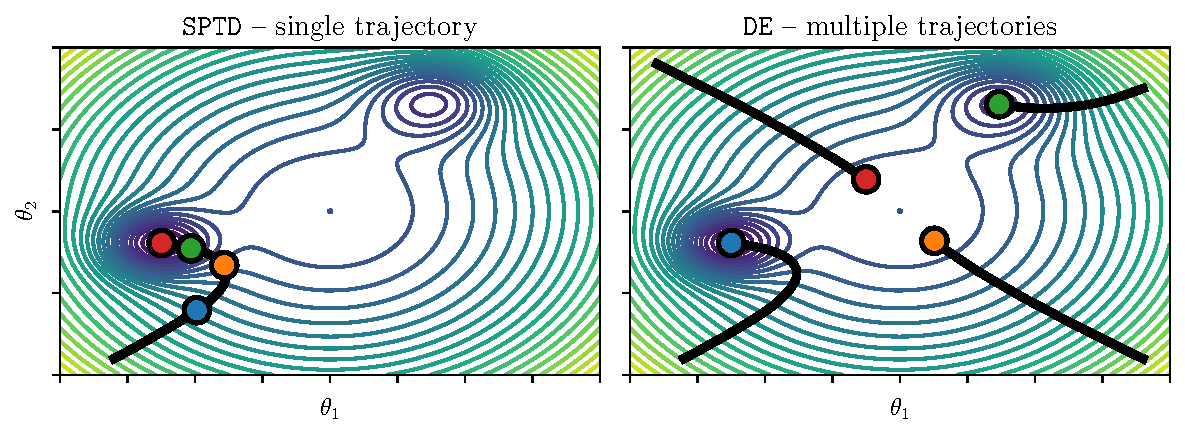
\includegraphics[width=\linewidth]{figs/sptd/sptd_de.pdf}
    \caption{\textbf{Illustrative comparison of \sptd and \de on a toy 2-D loss landscape}. \textit{Left}: a single SGD trajectory (black) descending into the bottom-left well, with four late-stage checkpoints highlighted in color to capture localized instability. \textit{Right}: four independent SGD runs (black) converging to multiple distinct minima, each marked by its final checkpoint (colored) to approximate global posterior modes.
}
    \label{fig:sptd_de_traj}
\end{figure}

\subsection{Deep Ensembles as Monte-Carlo Posterior Estimators}
\label{ssec:deep_ensembles_theory}

A complementary—and historically more popular—route to posterior variance is the \emph{Deep Ensemble} (\de) paradigm \citep{lakshminarayanan2017simple}.  
Here we train $M$ models $\{f_{\theta^{(m)}}\}_{m=1}^{M}$ from \emph{independent random initializations} (or data shuffles) and treat their empirical distribution as a Monte-Carlo approximation of the Bayesian posterior:
\begin{equation}
  \hat{p}_{\textsc{de}}(\theta)
  \;=\;
  \frac1M\sum_{m=1}^{M}\delta_{\theta^{(m)}}, 
  \quad\Longrightarrow\quad
  \operatorname{Var}_{\hat{p}_{\textsc{de}}}\bigl[f_{\theta}(\bm{x})\bigr]
  \;=\;
  \frac1M\sum_{m}\Bigl\lVert
      f_{\theta^{(m)}}(\bm{x})
      - \bar{f}(\bm{x})
  \Bigr\rVert^{2},
\end{equation}
with $\bar{f}(\bm{x})$ the ensemble mean.  
This variance estimator carries the same uncertainty semantics as the checkpoint-instability score $g(\bm{x})$, but differs in \emph{where} the Monte-Carlo samples come from:

\begin{center}
\begin{tabular}{p{0.23\linewidth}p{0.34\linewidth}p{0.34\linewidth}}
\toprule
 & \textbf{Sampling mechanism} & \textbf{Typical computational cost} \\
\midrule
\textbf{Deep Ensembles} & Independent SGD runs sample \emph{between} basins. & $\mathcal{O}(M)$ training + $\mathcal{O}(M)$ inference.\\[2pt]
\textbf{Selective Prediction Training Dyanmics} & One SGD run, checkpoints sample \emph{within} a basin. & $\mathcal{O}(1)$ training\footnotemark{} + $\mathcal{O}(T)$ inference ($T\le50$).\\
\bottomrule
\end{tabular}
\end{center}
\footnotetext{Aside from negligible checkpoint storage, \sptd\ does not increase training time.}

\paragraph{When do the two (dis-)agree?}  
If the posterior is \emph{multi-modal} (several distant basins with comparable posterior mass), \de captures variance \emph{between} modes, whereas checkpoints mainly capture \emph{local} variance inside one basin. We illustrate this behavior in Figure~\ref{fig:sptd_de_traj}. It is also possible to combine both approaches (\sptdde) which yields a near-superset of posterior support. We explore this choice in our experiments in Section~\ref{sec:emp_eval}. Together, checkpoints and ensembles represent two sides of the same Bayesian coin—local versus global exploration of the posterior landscape.  Understanding their relationship clarifies why their judicious combination delivers the best empirical coverage–utility balance.

\subsection{Limitations and Practical Implications}

While the argument above justifies the use of training dynamics, several caveats deserve attention:

\begin{itemize}
  \item \textbf{Diminished model diversity.}  Extremely over-parameterized networks or aggressive learning-rate schedules can lead SGD to converge to almost identical solutions, weakening the disagreement signal.  In such cases one can (i)~retain more checkpoints, (ii)~restart training with different data shuffles, or (iii)~combine \sptd\ with lightweight ensemble members.
  \item \textbf{Curriculum or non-stationary data.}  If the data distribution changes during training, early checkpoints reflect a different task than later ones.  Fixed data ordering or replay buffers help ensure that disagreement genuinely reflects uncertainty rather than curriculum artefacts.
  \item \textbf{Calibration needs.}  The raw instability scores are \emph{rank-consistent} with risk but need post-hoc calibration (e.g.\ isotonic regression) when probabilistic coverage guarantees are required.
\end{itemize}

Having established the theoretical underpinnings and practical scope of \sptd, we next evaluate its performance across classification, regression, and forecasting tasks.


\section{Empirical Evaluation}
\label{sec:emp_eval}

We present a comprehensive empirical study demonstrating the effectiveness of \sptd across domains. Our results show that computing and thresholding the proposed weighted instability score from \sptd provides a strong score for selective classification, regression, and time series prediction.

\subsection{Classification}

\paragraph{Key Research Goals.} As part of our experiments we:
\begin{itemize}
    \item Study the accuracy/coverage trade-off with comparison to past work, showing that \sptd outperforms existing work.
    \item Present exemplary training-dynamics-derived label evolution curves for individual examples from all datasets.
    \item Examine our method's sensitivity to the checkpoint selection strategy and the weighting parameter~$k$.
    \item Evaluate the detection performance of out-of-distribution and adversarial examples, showing that \sptd can be applied beyond the i.i.d. assumption of selective prediction.
    \item Provide a detailed cost vs performance tradeoff of \sptd and competing SP methods.
    \item Analyze distributional training dynamics patterns of both correct and incorrect data points, the separation of which enables performative selective classification.
\end{itemize} 

\paragraph{Datasets \& Training.} We evaluate \sptd on vision benchmarks that are common in the selective classification literature: CIFAR-10/CIFAR-100~\citep{krizhevsky2009learning}, StanfordCars~\citep{krause20133d}, and Food101~\citep{bossard14}. For each dataset, we train a deep neural network following the ResNet-18 architecture~\citep{he2016deep} and checkpoint each model after processing $50$ mini-batches of size $128$. All models are trained over $200$ epochs ($400$ epochs for StanfordCars) using the SGD optimizer with an initial learning rate of $10^{-2}$, momentum $0.9$, and weight decay $10^{-4}$. Across all datasets, we decay the learning rate by a factor of $0.5$ in $25$-epoch intervals.

\paragraph{Baselines.} We compare our method (\sptd) to common SC techniques previously introduced in Section~\ref{sec:background_sptd}: Softmax Response (\sr) and Self-Adaptive Training (\sat). Based on recent insights from~\cite{feng2023towards}, we (i) train \sat with additional entropy regularization\footnote{This entropy regularization step is designed to encourage the model to be more confident in its predictions.}; and (ii) derive \sat's score by applying Softmax Response (\sr) to the underlying classifier (instead of thresholding the abstention class). We refer to this method as \satersr. We do not include results for SelectiveNet, Deep Gamblers, or Monte-Carlo Dropout as previous works~\citep{huang2020self,feng2023towards} have shown that \fixed{\satersr} strictly dominates these methods. In contrast to recent SC works, we do however include results \fixed{with} Deep Ensembles (\de)~\citep{balaji2017uncertainty}, a relevant baseline from the uncertainty quantification literature. Our hyper-parameter tuning procedure is documented in Appendix~\ref{app:baseline_hyperparams}.

\paragraph{Accuracy/Coverage Trade-off.} Consistent with standard evaluation schemes for selective classification, our main experimental results examine the accuracy/coverage trade-off of \sptd. We present our performance results with comparison to past work in Table~\ref{tab:target_cov} where we demonstrate \sptd's effectiveness on CIFAR-10, CIFAR-100, StanfordCars, and Food101. We document the results obtained by \sptd, \sat, \sr, and \de across the full coverage spectrum. We see that \sptd outperforms both \sat and \sr and performs similarly as \de. To further boost performance across the accuracy/coverage spectrum, we combine \sptd and \de by applying \sptd on each ensemble member from \de and then average their scores. More concretely, we estimate $\sptdde = \frac{1}{m}\sum_{m=1}^M \sptd_m$ where $\sptd_m$ computes $g$ on each ensemble member $m\in[M]$. This combination leads to new state-of-the-art selective classification performance and showcases that \sptd can be flexibly applied on top of established training pipelines. 
\newlyadded{
Further evidence towards this flexibility is provided in Appendix~\ref{sec:sptd_on_sat} where we show that applying \sptd on top of \sat also improves performance.
}

\begin{figure}[t]
\vspace{-5pt}
\centering

\begin{subfigure}[b]{0.23\linewidth}
  \centering
  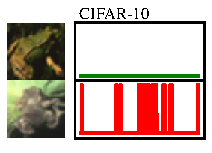
\includegraphics[width=\linewidth]{figs/sptd/cifar10_points.pdf}
  \caption{CIFAR-10}
\end{subfigure}
\hfill
\begin{subfigure}[b]{0.23\linewidth}
  \centering
  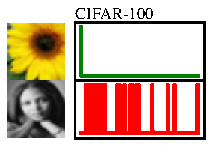
\includegraphics[width=\linewidth]{figs/sptd/cifar100_points.pdf}
  \caption{CIFAR-100}
\end{subfigure}
\hfill
\begin{subfigure}[b]{0.23\linewidth}
  \centering
  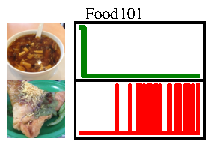
\includegraphics[width=\linewidth]{figs/sptd/food_points.pdf}
  \caption{Food-101}
\end{subfigure}
\hfill
\begin{subfigure}[b]{0.23\linewidth}
  \centering
  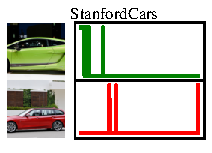
\includegraphics[width=\linewidth]{figs/sptd/cars_points.pdf}
  \caption{Stanford Cars}
\end{subfigure}

\caption[\textbf{Most characteristic examples across datasets.}]{\textbf{Most characteristic examples across datasets.} For each dataset, we show the samples with the most stable and most unstable (dis-)agreement with the final label along with their corresponding $a_t$ indicator function. Correct points are predominantly characterized by disagreements early in training while incorrect points change their class label throughout (but importantly close to the end of) training. We provide additional examples from all datasets in Figure~\ref{fig:indiv_ex_ext}.}
\label{fig:indiv_ex}
\end{figure}


\paragraph{Individual Evolution Plots.} To analyze the effectiveness of our disagreement metric proposed in Section~\ref{sec:method}, we examine the evolution curves of our indicator variable $a_t$ for individual datapoints in Figure~\ref{fig:indiv_ex}. In particular, for each dataset, we present the most stable and the most unstable data points from the test sets and plot the associated label disagreement metric $a_t$ over all checkpoints. We observe that easy-to-classify examples only show a small degree of oscillation while harder examples show a higher frequency of oscillations, especially towards the end of training. This result matches our intuition: our model should produce correct decisions on data points whose prediction is mostly constant throughout training and should reject data points for which intermediate models predict inconsistently. Moreover, as depicted in Figure~\ref{fig:scores}, we also show that our score $g(\cdot)$ yields distinct distributional patterns for both correctly and incorrectly classified points. This separation enables strong coverage/accuracy trade-offs via our thresholding procedure.

\begin{figure*}[t]
  \centering
  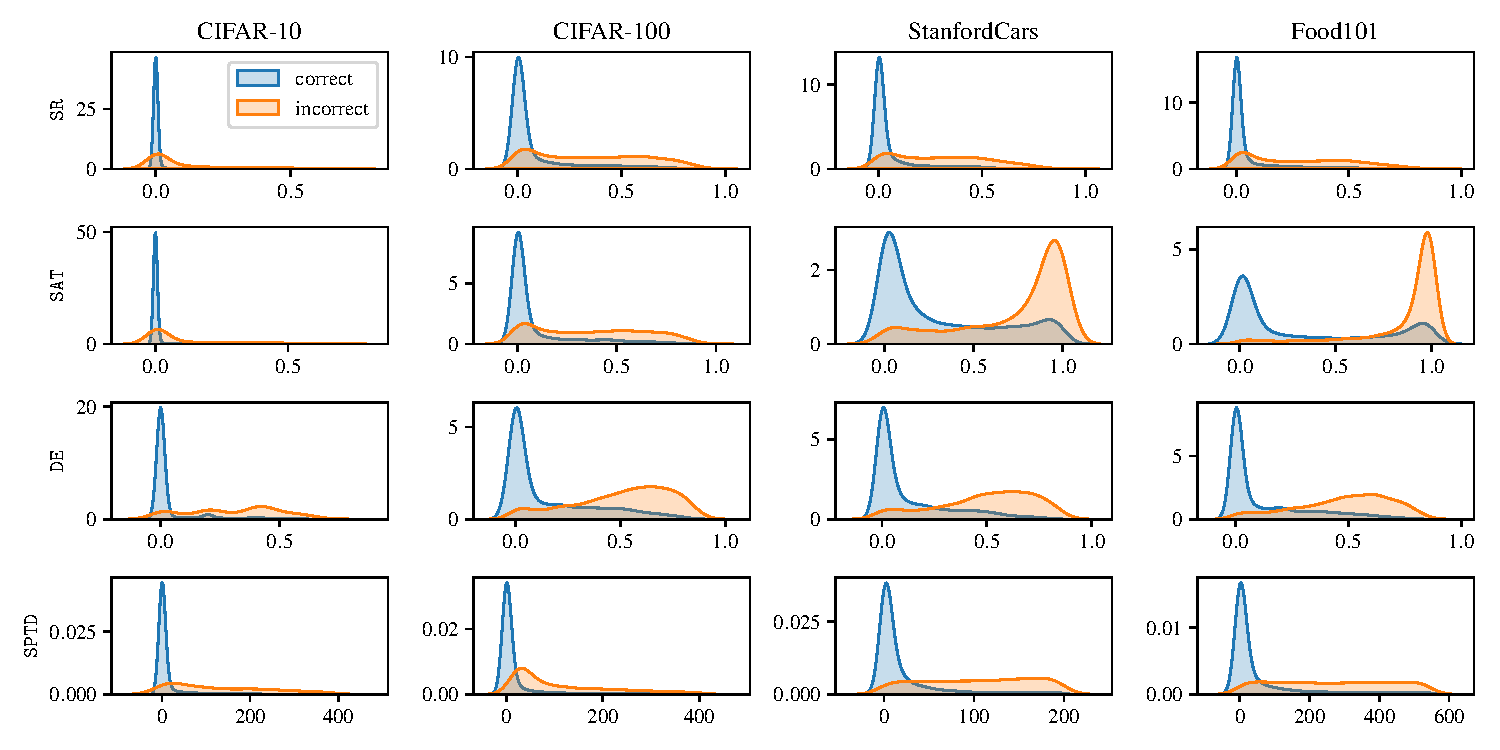
\includegraphics[width=\linewidth]{figs/sptd/g_dists.pdf}
\caption[Distribution of $g$ for different datasets and selective classification methods.]{\textbf{Distribution of $g$ for different datasets and selective classification methods.}  Since all methods are designed to address the selective prediction problem, they all manage to separate correct from incorrect points (albeit at varying success rates). We see that \sptd spreads the scores for incorrect points over a wide range with little overlap. We observe that for \sr, incorrect and correct points both have their mode at approximately the same location which hinders performative selective classification. Although \sat and \de show larger bumps at larger score ranges, the separation with correct points is weaker as correct points also result in higher scores more often than for \sptd. }
\label{fig:scores}
\end{figure*}

\begin{figure*}[t]
  \centering
  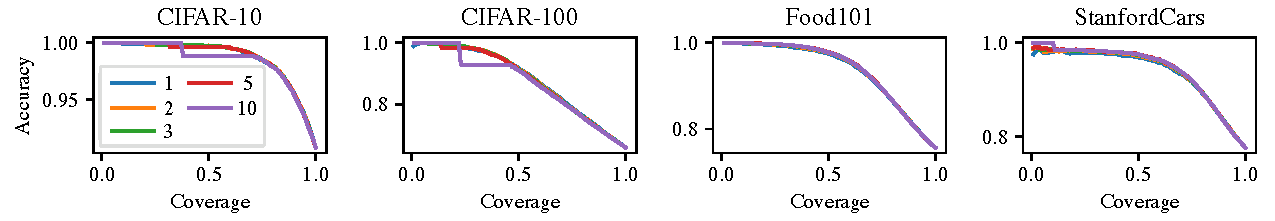
\includegraphics[width=\linewidth]{figs/sptd/k_ablation.pdf}
\caption[Coverage/error trade-off of \texttt{SPTD} for varying checkpoint weighting $k$ as used in $v_t$.]{\textbf{Coverage/error trade-off of \texttt{SPTD} for varying checkpoint weighting $k$ as used in $v_t$.} We observe strong performance for $k \in [1,3]$ across datasets.
}
\label{fig:weighting}
\end{figure*}

\paragraph{Checkpoint Weighting Sensitivity.} One important hyper-parameter of our method is the weighting of intermediate predictions. Recall from Section~\ref{sec:method} that \sptd approximates the expected stability for correctly classified points via a weighting function $v_t = (\frac{t}{T})^k$. In Figure~\ref{fig:weighting} in the Appendix, we observe  that \sptd is robust to the choice of $k$ and that \fixed{$k \in [1,3]$} performs best. At the same time, we find that increasing $k$ too much leads to a decrease in accuracy at medium coverage levels. This result emphasizes that (i)~large parts of the training process contain valuable signals for selective classification; and that (ii)~early label disagreements arising at the start of optimization should be de-emphasized by our method.

\begin{figure*}[t]
  \centering
  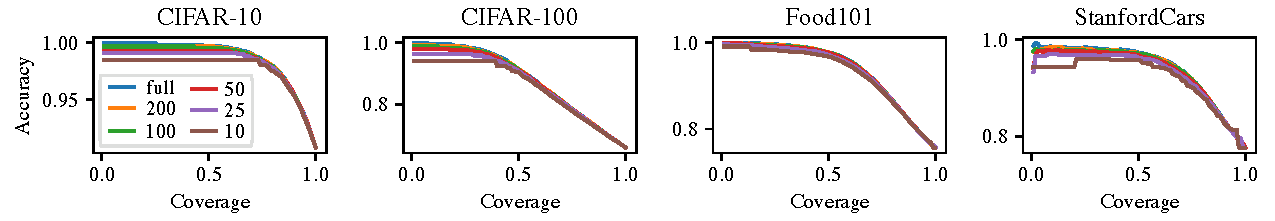
\includegraphics[width=\linewidth]{figs/sptd/checkp_ablation.pdf}
\caption[Coverage/error trade-off of \texttt{SPTD} for varying checkpoint counts.]{\textbf{Coverage/error trade-off of \texttt{SPTD} for varying checkpoint counts}. \sptd delivers consistent performance independent of the checkpointing resolution at high coverage. At low coverage, a more detailed characterization of training dynamics helps.
}
\label{fig:resolution}
\end{figure*}

\paragraph{Checkpoint Selection Strategy.} The second important hyper-parameter of our method is the checkpoint selection strategy. In particular, to reduce computational cost, we study the sensitivity of \sptd with respect to the checkpointing resolution in Figure~\ref{fig:resolution}. Our experiments demonstrate favorable coverage/error trade-offs between $25$ and $50$ checkpoints when considering the full coverage spectrum. However, when considering the high coverage regime in particular (which is what most selective prediction works focus on), even sub-sampling $10$ intermediate models is sufficient for SOTA selective classification. Hence, with only observing the training stage, our method's computational overhead reduces to only $10$ forward passes at test time when the goal is to reject at most $30\%-50\%$ of incoming data points. In contrast, \de requires to first train $E$ models (with $E=10$ being a typical and also our particular choice for \de) and perform inference on these $E$ models at test time. Further increasing the checkpointing resolution does offer increasingly diminishing returns but also leads to improved accuracy-coverage trade-offs, especially at low coverage.

\begin{figure*}[t]
  \centering
  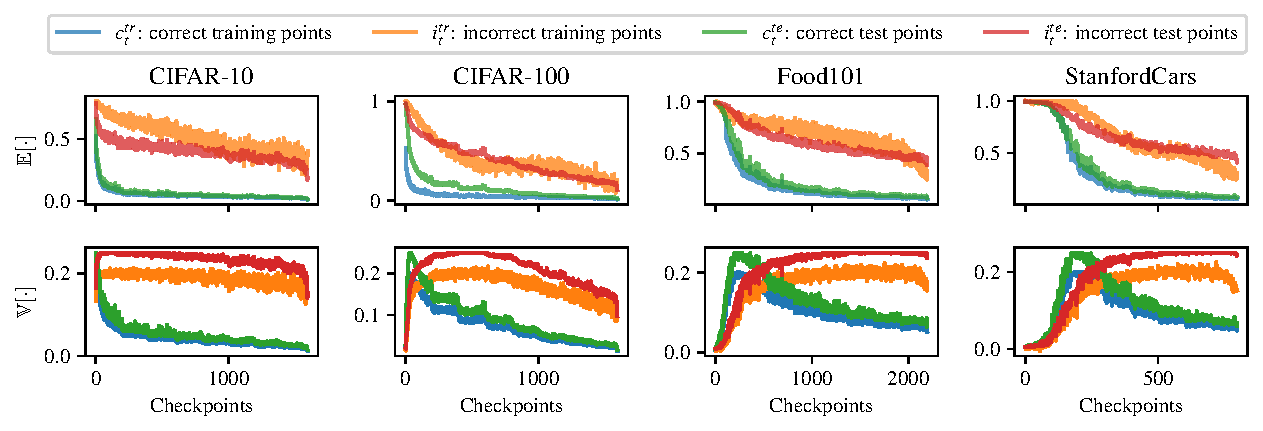
\includegraphics[width=\linewidth]{figs/sptd/et_vt_updated.pdf}
\caption[Monitoring expectations and variances for correct/incorrect training and test points.]{\textbf{Monitoring expectations $\mathbb{E}[\cdot]$ and variances $\mathbb{V}[\cdot]$ for correct/incorrect training and test points}. We observe that correctly classified points (cold colors) have both their expectations and variances quickly decreasing to 0 as training progresses. Incorrectly classified points (warm colors) both exhibit large expectations and variances and stay elevated over large periods.}
\label{fig:exp_var_trends}
\end{figure*}


\paragraph{Examining the Convergence Behavior of Training and Test Points.}

The effectiveness of \sptd relies on our hypothesis that correctly classified points and incorrectly classified points exhibit distinct training dynamics. We verify this hypothesis in Figure~\ref{fig:exp_var_trends} where we examine the convergence behavior of the disagreement distributions of correct ($c^\text{tr}_t$) / incorrect ($i^\text{tr}_t$) training and correct ($c^\text{te}_t$) / incorrect ($i^\text{te}_t$) test points. We observe that the expected disagreement for both correctly classified training $c^\text{tr}_t$ and test points $c^\text{te}_t$ points converge to $0$ over the course of training. The speed of convergence is subject to the difficulty of the optimization problem with more challenging datasets exhibiting slower convergence in predicted label disagreement. We also see that the variances follow an analogous decreasing trend. This indicates that correctly classified points converge to the final label quickly and fast convergence is strongly indicative of correctness. Furthermore, the overlap suggests that correct test points are more likely to be forgeable as their dynamics look indistinguishable to correct training points (recall Section~\ref{sec:forging} on the connection between our method and forging). In contrast, incorrectly classified points $i^\text{tr}_t$ and $i^\text{te}_t$ show significantly larger mean and variance levels. This clear separation in distributional evolution patterns across correct and incorrect points leads to strong selective prediction performance in our \sptd framework.

\label{sec:ts_exp}
\begin{figure*}[t]
    \centering
    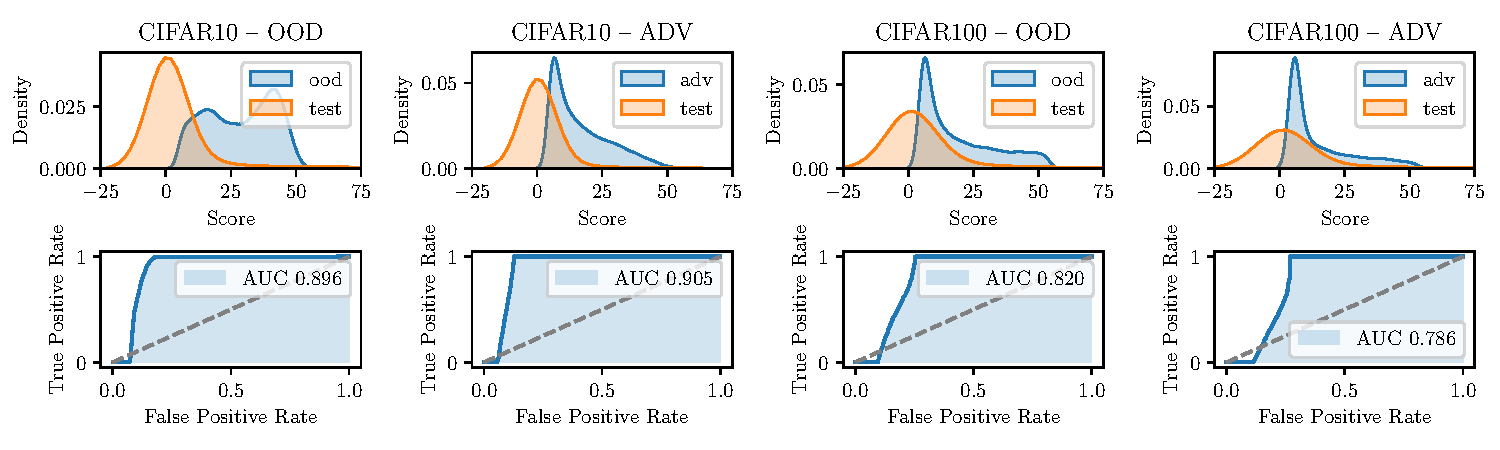
\includegraphics[width=\linewidth]{figs/sptd/adv_ood.pdf}
    \caption[Performance of \sptd on out-of-distribution (OOD) and adversarial sample detection.]{\textbf{Performance of \sptd on out-of-distribution (OOD) and adversarial sample detection}. The first row shows the score distribution of the in-distribution CIFAR-10/100 test set vs the SVHN OOD test set or a set consisting of adversarial samples generated via a PGD attack in the final model. The second row shows the effectiveness of a thresholding mechanism by computing the area under the ROC curve. Our score enables separation of anomalous data points from in-distribution test points.}
    \label{fig:adv_ood}
\end{figure*}

\paragraph{Detection of Out-of-Distribution and Adversarial Examples.}

Out-of-distribution (OOD) and adversarial example detection are important disciplines in trustworthy ML related to selective prediction. We therefore provide preliminary evidence in Figure~\ref{fig:adv_ood} that our method can be used for detecting OOD and adversarial examples. While these results are encouraging, we remark that adversarial and OOD samples are less well defined as incorrect data points and can come in a variety of different flavors (\ie various kinds of attacks or various degrees of OOD-ness). As such, we strongly believe that future work is needed to determine whether a training-dynamics-based approach to selective prediction can be reliably used for OOD and adversarial sample identification. 

\paragraph{Cost vs Performance Tradeoff.} 

In Table~\ref{tab:cost}, we report both the time and space complexities for all SC methods at training and test time along with their selective classification performance as per our results in Table~\ref{tab:target_cov} and Figure~\ref{fig:resolution}. We denote with $E$ the number of  \de models and with $T$ the number of \sptd checkpoints. Although \sr and \sat are the cheapest methods to run, they also perform the poorest at SC. \sptd is significantly cheaper to train than \de and achieves competitive performance at $T \approx E$. Although \sptdde is the most expensive model, it also provides the strongest performance.

\begin{table}[ht]
\tabcolsep=0.12cm
\small
    \centering 
     \begin{tabular}{cccccc} 
     \toprule
     Method & Train Time & Train Space & Inf Time & Inf Space & Rank \\ 
     \midrule
     \sr & $O(1)$ & $O(1)$ & $O(1)$ & $O(1)$ & 5 \\
     \sat & $O(1)$ & $O(1)$ & $O(1)$ & $O(1)$ & 4 \\
     \de & $O(E)$ & $O(E)$ & $O(E)$ & $O(E)$ & =2 \\
     \sptd & $O(1)$ & $O(T)$ & $O(T)$ & $O(T)$ & =2 \\
     \sptdde & $O(E)$ & $O(ET)$ & $O(ET)$ & $O(ET)$ & 1\\ 
     \bottomrule
    \end{tabular}
    \caption[Cost vs performance tradeoff in terms of training time/space, inference time/space and the performance rank.]{\textbf{Cost vs performance tradeoff in terms of training time/space, inference time/space and the performance rank.} \sptd is comparable in performance (at $T \approx E$) and cheaper to train than \de. \sptdde is the most expensive model, but delivers the best performance across datasets.}
    \label{tab:cost}
\end{table}

\begin{figure*}[t]
    \centering
    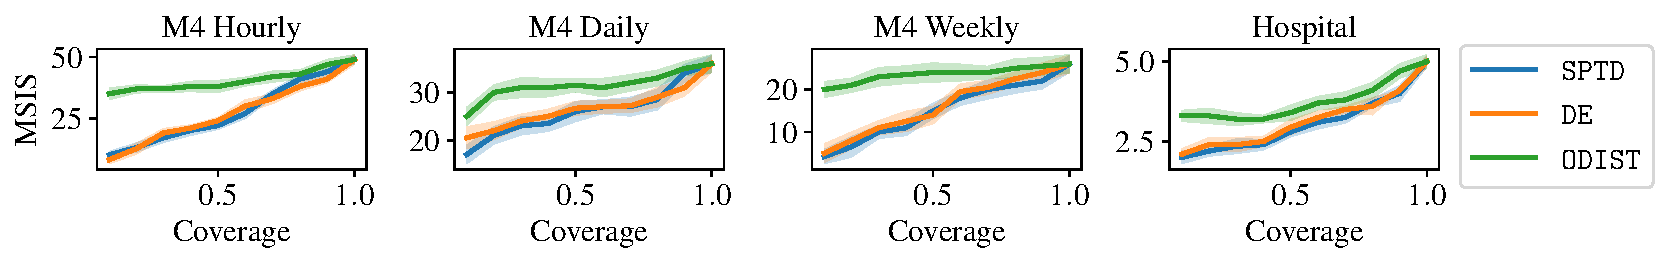
\includegraphics[width=0.97\linewidth]{figs/sptd/ts.pdf}
    \caption[MSIS/coverage trade-off across various time series prediction datasets.]{\textbf{MSIS/coverage trade-off across various time series prediction datasets}. \sptd offers comparable performance to \de but provides improved results at low coverage.}
    \label{fig:ts}
\end{figure*}

\subsection{Regression Experiments}
\label{sec:regr_exp}

\begin{figure*}[t]
    \centering
    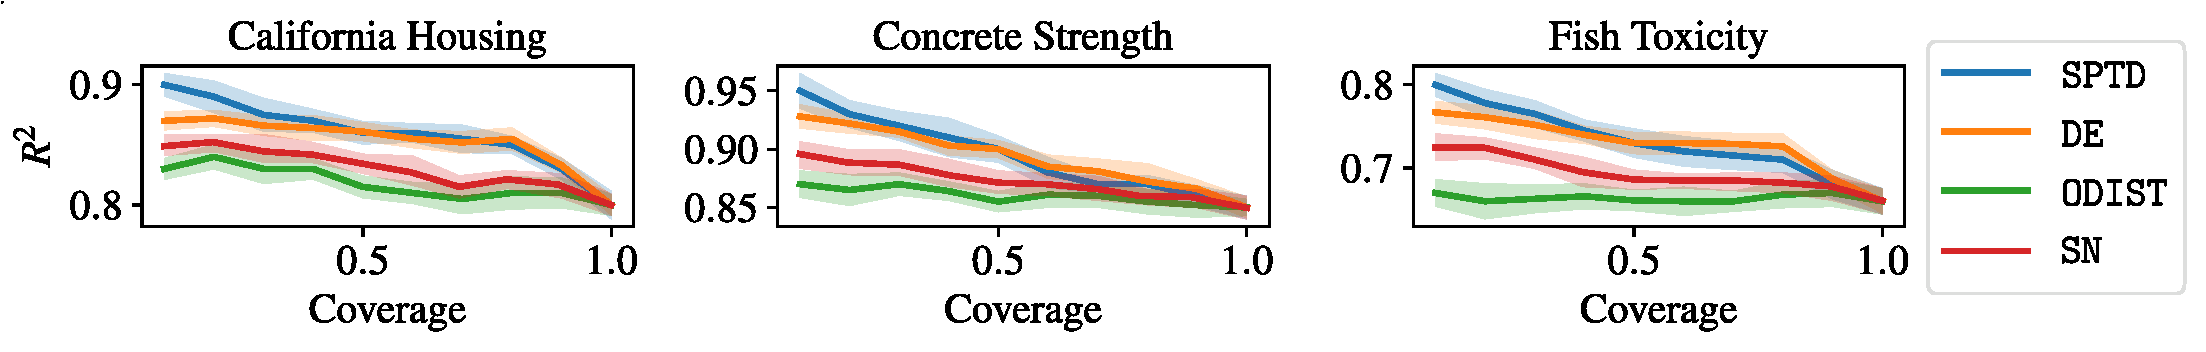
\includegraphics[width=0.97\linewidth]{figs/sptd/regr_sn.pdf}
    \caption[$R^2$/coverage trade-off across various regression datasets.]{\textbf{$R^2$/coverage trade-off across various regression datasets}. \sptd offers comparable performance to \de but provides improved results at low coverage.}
    \label{fig:regr}
\end{figure*}

\paragraph{Datasets.} Our experimental suite for regression considers the following datasets: %\anvith{any reference for why these datasets?}: the 
California housing dataset~\citep{pace1997sparse} ($N=20640$, $D=8$), the concrete strength dataset~\citep{misc_concrete_compressive_strength_165} ($N=1030$, $D=9$), and the fish toxicity dataset~\citep{misc_qsar_fish_toxicity_504} ($N=546$, $D=9$). 

\paragraph{Model Setup \& Baselines.} We split all datasets into $80\%$ training and $20\%$ test sets after a random shuffle. Then, we train a fully connected neural network with layer dimensionalities $D \rightarrow 10 \rightarrow 7 \rightarrow 4 \rightarrow 1$. Optimization is performed using full-batch gradient descent using the Adam optimizer with learning rate $10^{-2}$ over $200$ epochs and weight decay $10^{-2}$. We consider the following baseline methods for rejecting input samples: (i) approximating the predictive variance using deep ensembles (\de) \citep{balaji2017uncertainty, zaoui2020regression}; (ii) SelectiveNet (\sn) which explicitly optimizes utility given a desired coverage constraint; and (iii) training the model with a Gaussian parametric output distribution (\odist) via maximum likelihood maximization \citep{alexandrov2019gluonts}.

\paragraph{Main Results.} We document our results in Figure~\ref{fig:regr}. We see that the \odist only delivers subpar results (likely due to mis-calibration) and does not provide a meaningful signal for selective prediction. On the other hand, \de and \sptd perform comparably with \sptd outperforming \de at low coverage. We stress again that \sptd's training cost is significantly cheaper than \de's while matching the inference-time cost when sub-sampling a reduced set of checkpoints. 

\subsection{Time Series Experiments}
\label{sec:ts_exp}

\paragraph{Datasets.} As part of our time series experiments, we mainly consider the M4 forecasting competition dataset~\citep{makridakis2020m4} which contains time series aggregated at various time intervals (\eg hourly). In addition, we also provide experimentation on the Hospital dataset~\citep{hyndman2015expsmooth}.

\paragraph{Models \& Setup.} Our experimentation is carried out using the GluonTS time series framework~\citep{alexandrov2019gluonts} and the DeepAR model \citep{salinas2020deepar}, a recurrent neural network designed for time series forecasting. We train all models over 200 epochs and evaluate performance using the mean scaled interval score (MSIS) performance metric~\citep{makridakis2020m4}. Our baselines correspond to the same as presented for regression in Section~\ref{sec:regr_exp}: deep ensembles (\de), and output parameterization using a Student-t distribution (\odist).

\paragraph{Main Results.} Our time series results are shown in Figure~\ref{fig:ts} and are consistent with our results for regression: \odist does not provide a meaningful signal for selective prediction while \sptd and \de perform similarly well. \sptd further improves results over \de at low converge.


\begin{table*}[h!]
\fontsize{7.5}{10}\selectfont
\tabcolsep=0.2cm
    \centering {
    \begin{tabular}{ccccccc}
\toprule
&  Coverage &       \sr &       \fixed{\satersr} &      \de &      \sptd &        \sptdde \\
\midrule
 \multirow{10}{*}{\rotatebox[origin=c]{90}{\textit{CIFAR-10}}} &       100 &  \underline{\bfseries 92.9 (±0.0)} & \underline{\bfseries 92.9 (±0.0)} & \bfseries 92.9 (±0.0) & \underline{\bfseries 92.9 (±0.0)} & \bfseries 92.9 (±0.1) \\
  &        90 &  \underline{96.4 (±0.1)} &  96.3 (±0.1) &  \bfseries 96.8 (±0.1) &  \underline{96.5 (±0.0)} &  \bfseries 96.7 (±0.1) \\
  &        80 &  98.1 (±0.1) &  98.1 (±0.1) &  \bfseries 98.7 (±0.0) &  \underline{98.4 (±0.1)} &  \bfseries 98.8 (±0.1) \\
  &        70 &  98.6 (±0.2) &  99.0 (±0.1) &  \bfseries 99.4 (±0.1) &  \underline{99.2 (±0.0)} &  \bfseries 99.5 (±0.0) \\
  &        60 &  98.7 (±0.1) &  99.4 (±0.0) &  99.6 (±0.1) &  \underline{\bfseries 99.6 (±0.2)} &  \bfseries 99.8 (±0.0) \\
  &        50 &  98.6 (±0.2) &  \underline{99.7 (±0.1)} &  99.7 (±0.1) &  \underline{99.8 (±0.0)} &  \bfseries 99.9 (±0.0) \\
  &        40 &  98.7 (±0.0) &  \underline{99.7 (±0.0)} &  99.8 (±0.0) &  \underline{99.8 (±0.1)} & \bfseries 100.0 (±0.0) \\
  &        30 &  98.5 (±0.0) &  \underline{99.8 (±0.0)} &  99.8 (±0.0) &  \underline{99.8 (±0.1)} & \bfseries 100.0 (±0.0) \\
  &        20 &  98.5 (±0.1) &  \underline{99.8 (±0.1)} &  99.8 (±0.0) & \underline{\bfseries 100.0 (±0.0)} & \bfseries 100.0 (±0.0) \\
  &        10 &  98.7 (±0.0) &  99.8 (±0.1) &  99.8 (±0.1) & \underline{\bfseries 100.0 (±0.0)} & \bfseries 100.0 (±0.0) \\
 \midrule
  \multirow{10}{*}{\rotatebox[origin=c]{90}{\textit{CIFAR-100}}}  &       100 &  \underline{\bfseries 75.1 (±0.0)} &  \underline{\bfseries 75.1 (±0.0)} &  \bfseries 75.1 (±0.0) &  \underline{\bfseries 75.1 (±0.0)} &  \bfseries 75.1 (±0.0) \\
& 90 & 78.2 (± 0.1) & 78.9 (± 0.1) & 80.2 (± 0.0) & \underline{80.4 (± 0.1)} & \bfseries 81.1 (± 0.1) \\
& 80 & 82.1 (± 0.0) & 82.9 (± 0.0) & 84.7 (± 0.1) & \underline{84.6 (± 0.1)} & \bfseries 85.0 (± 0.2) \\
& 70 & 86.4 (± 0.1) & 87.2 (± 0.1) & 88.6 (± 0.1) & \underline{\textbf{88.7 (± 0.0)}} & \bfseries 88.8 (± 0.1) \\
& 60 & 90.0 (± 0.0) & 90.3 (± 0.2) & 90.2 (± 0.2) & \underline{90.1 (± 0.0)} & \bfseries 90.4 (± 0.1) \\
& 50 & 92.9 (± 0.1) & 93.3 (± 0.0) & 94.8 (± 0.0) & \underline{94.6 (± 0.0)} & \bfseries 94.9 (± 0.0) \\
& 40 & 95.1 (± 0.0) & 95.2 (± 0.1) & \textbf{96.8 (± 0.1)} & \underline{\textbf{96.9 (± 0.1)}} & \bfseries 96.9 (± 0.0) \\
& 30 & 97.2 (± 0.2) & 97.5 (± 0.0) & \textbf{98.4 (± 0.1)} & \underline{\textbf{98.4 (± 0.1)}} & \bfseries 98.5 (± 0.0) \\
& 20 & 97.8 (± 0.1) & 98.3 (± 0.1) & \textbf{99.0 (± 0.0)} & \underline{98.8 (± 0.2)} & \bfseries 99.2 (± 0.1) \\
& 10 & 98.1 (± 0.0) & 98.8 (± 0.1) & 99.2 (± 0.1) & \underline{\textbf{99.4 (± 0.1)}} & \bfseries 99.6 (± 0.1) \\
\midrule

    \multirow{10}{*}{\rotatebox[origin=c]{90}{\textit{Food101}}} &       100 &  \underline{\bfseries 81.1 (±0.0)} &  \underline{\bfseries 81.1 (±0.0)} & \bfseries  81.1 (±0.0) & \underline{\bfseries 81.1 (±0.0)} & \bfseries 81.1 (±0.0) \\
     &        90 &  85.3 (±0.1) &  85.5 (±0.2) &  86.2 (±0.1) &  \underline{85.7 (±0.0)} &  \bfseries 86.7 (±0.0) \\
     &        80 &  87.1 (±0.0) &  89.5 (±0.0) &  90.3 (±0.0) &  \underline{89.9 (±0.0)} &  \bfseries 91.3 (±0.1) \\
     &        70 &  92.1 (±0.1) &  92.8 (±0.1) &  \bfseries 94.5 (±0.1) &  \underline{93.7 (±0.0)} &  \bfseries 94.6 (±0.0) \\
     &        60 &  95.2 (±0.1) &  95.5 (±0.1) &  \bfseries 97.0 (±0.0) &  \underline{\bfseries 97.0 (±0.0)} &  \bfseries 97.0 (±0.0) \\
     &        50 &  97.3 (±0.1) &  97.5 (±0.0) &  98.2 (±0.0) &  \underline{\bfseries98.3 (±0.2)} &  \bfseries 98.5 (±0.0) \\
     &        40 &  98.7 (±0.0) &  98.7 (±0.2) &  \bfseries 99.1 (±0.0) &  \underline{99.1 (±0.1)} &  \bfseries 99.2 (±0.1) \\
     &        30 &  99.5 (±0.0) &  99.7 (±0.2) &  99.2 (±0.0) &  \underline{99.6 (±0.0)} &  \bfseries 99.7 (±0.0) \\
     &        20 &  99.7 (±0.1) &  99.7 (±0.2) &  \bfseries 99.9 (±0.1) &  \underline{\bfseries 99.8 (±0.0)} &  \bfseries 99.9 (±0.1) \\
     &        10 &  99.8 (±0.0) &  99.8 (±0.1) &  \bfseries 99.9 (±0.1) &  \underline{\bfseries 99.9 (±0.1)} &  \bfseries 99.9 (±0.1) \\
  \midrule
    \multirow{10}{*}{\rotatebox[origin=c]{90}{\textit{StanfordCars}}} &       100 & \bfseries \underline{77.6 (±0.0)} & \underline{\bfseries 77.6 (±0.0)} & \bfseries 77.6 (±0.0) & \underline{\bfseries 77.6 (±0.0)} & \bfseries 77.6 (±0.0) \\
     &        90 &  83.0 (±0.1) &  83.0 (±0.2) &  \bfseries 83.7 (±0.1) &  \underline{83.3 (±0.1)} &  \bfseries 83.7 (±0.2) \\
     &        80 &  87.6 (±0.0) &  88.0 (±0.1) &  88.7 (±0.1) &  \underline{\bfseries 89.3 (±0.0)} &  \bfseries 89.7 (±0.0) \\
     &        70 &  90.8 (±0.0) &  92.2 (±0.1) &  92.4 (±0.1) &  \underline{\bfseries 93.6 (±0.0)} &  93.4 (±0.1) \\
     &        60 &  93.5 (±0.1) &  95.2 (±0.1) &  95.3 (±0.0) &  \underline{\bfseries 96.2 (±0.0)} &  \bfseries 96.3 (±0.0) \\
     &        50 &  95.3 (±0.0) &  \underline{96.9 (±0.2)} &  96.4 (±0.1) &  \underline{\bfseries 97.0 (±0.1)} &  \bfseries 97.1 (±0.3) \\
     &        40 &  96.8 (±0.0) &  \underline{97.8 (±0.0)} &  \bfseries 97.8 (±0.2) &  \underline{\bfseries 97.8 (±0.1)} &  \bfseries 97.8 (±0.0) \\
     &        30 &  97.5 (±0.1) &  \underline{98.2 (±0.2)} &  \bfseries 98.6 (±0.0) &  \underline{98.2 (±0.2)} &  \bfseries 98.9 (±0.0) \\
     &        20 &  98.1 (±0.0) &  \underline{98.4 (±0.1)} &  \bfseries 98.9 (±0.2) &  \underline{98.6 (±0.0)} &  \bfseries 99.0 (±0.0) \\
     &        10 &  98.2 (±0.1) &  \underline{98.7 (±0.1)} &  \bfseries 99.5 (±0.1) &  \underline{98.5 (±0.1)} &  \bfseries 99.5 (±0.0) \\
\bottomrule
\end{tabular}
\caption[Selective accuracy achieved across coverage levels]{\textbf{Selective accuracy achieved across coverage levels}. We find that \texttt{SPTD}-based methods outperform current SOTA error rates across multiple datasets with full-coverage accuracy alignment. Numbers are reported with mean values and standard deviation computed over 5 random runs. \textbf{Bold} numbers are best results at a given coverage level across all methods and \underline{underlined} numbers are best results for methods relying on a single training run only. Datasets are consistent with~\cite{feng2023towards}.}
    \label{tab:target_cov}
    }
\end{table*} 

\section{Conclusion}

In this work we have proposed \sptd, a selective prediction technique that relies on measuring prediction instability of test points over intermediate model states obtained during training. Our method offers several advantages over previous works. In particular (i) it can be applied to all existing models whose checkpoints were recorded (hence the potential for immediate impact); (ii) it is composable with existing selective prediction techniques; (iii) it can be readily applied to both discrete and real-valued prediction problems; and (iv) it is more computationally efficient than competing ensembling-based approaches. We verified the performance of \sptd using an extensive empirical evaluation, leading to new state-of-the-art performance in the field. Beyond our work, we expect training dynamics information to be useful for identifying and mitigating other open problems in trustworthy machine learning such as (un)fairness, privacy, and model interpretability.